\subsection{Sitio de trabajo}
\subsubsection{Descripción}
El siguiente experimento se realizó en un contexto de ámbito laboral. Se analizó la red durante aproximadamente 20 minutos con la herramienta desarrollada para este trabajo, con el objetivo de obtener información que permita determinar las características de la misma con cierto respaldo empírico. Primero se presentarán los resultados obtenidos mediante gráficos y figuras, posteriormente se discutirán estos resultados para así arribar al fin antes mencionado.
 
\subsubsection{Resultados}
\begin{figure}[H]
  \centering	
	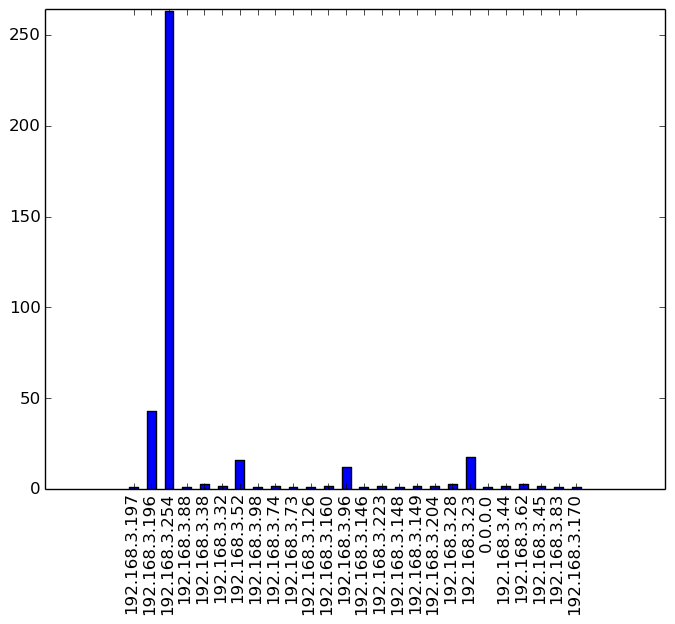
\includegraphics[scale=0.66]{../experimentacion-agarassino/histogram_src.png}
  \caption{Histograma de las IP fuente.}
	\label{fig:histo-src-sitiotrabajo}
\end{figure}

\begin{figure}[H]
  \centering	
	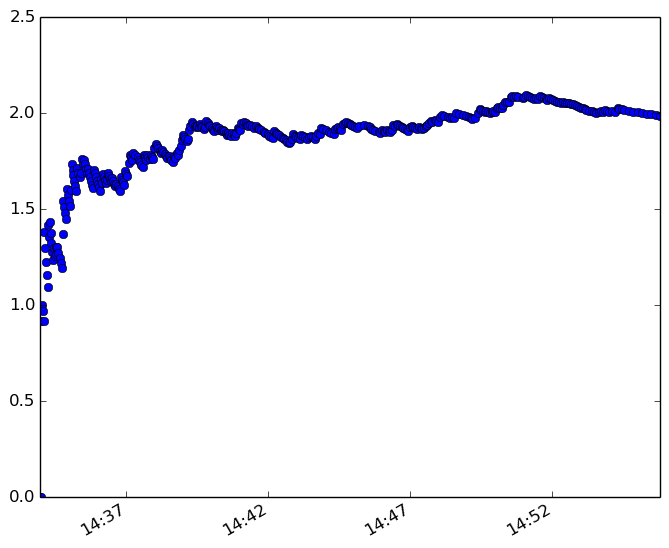
\includegraphics[scale=0.66]{../experimentacion-agarassino/entropy_src.png}
  \caption{Entropía en función del tiempo tomando como fuente de información las IP fuente.}
	\label{fig:entropia-src-sitiotrabajo}
\end{figure}

\subsubsection{Conclusiones del experimento}
La figura \ref{fig:histo-src-sitiotrabajo}, nos permite afirmar con suficiente confianza que la IP $192.168.3.254$ está asociada a un dispositivo de gran importancia para la red. Probablemente el dispositivo se trate de un router, que necesita averiguar constantemente las MAC asociadas a las computadoras en la red para poder retransmitir los paquetes dirigidas a estas de forma exitosa. Un grafo con los diversos agentes involucrados en la red, conectados a través de aristas representando la comunicación a través de paquetes ARP como se describió anteriormente, se puede hallar junto a este informe. La figura no se imprimió dentro de este mismo documento debido a su gran tamaño, pero observándolo esta última conclusión parece ser más fácil de dilucidar. 

Por otro lado, observando el gráfico de la entropía en función del tiempo en la figura \ref{fig:entropia-src-sitiotrabajo} se puede ver como en un principio, al poseer pocos datos sobre la fuente de información, la entropía parece oscilar sin aportar ningún dato de interés. A medida que transcurre el tiempo esta parece converger a un resultado cercano a 2. Sabiendo que la entropía se encuentra medida en bits, podemos afirmar que se encuentra acotada superiormente por $\log_{2}(n)$, en este caso la cantidad de símbolos involucrados es igual a la cantidad de IP's fuente en los paquetes ARP \textit{who-has}, es decir 26.  Por lo tanto la entropía será a lo sumo de aproximadamente $4,7$, dándonos un panorama un poco mejor de la posición en donde se encuentra parada la entropía de la red.